\section{Strongly Coupled Dark Matter}\label{sec:darkqcd}

\subsection{Background}\label{subsec:dmbkg}

Many astronomical observations, from various independent and complementary sources,
indicate that dark matter exists, comprises the majority of matter in the universe, and does not consist of any SM particles.
These sources include:
galaxy rotation curves~\cite{Rubin:1980zd,Persic:1995ru,vanDokkum:2018vup,PinaMancera:2021wpc};
strong~\cite{Clowe:2006eq} and weak~\cite{Chang:2017kmv} gravitational lensing;
the cosmic microwave background power spectrum~\cite{Planck:2018vyg} and the matter power spectrum of the universe~\cite{Dodelson:2011qv,Planck:2018nkj};
and discrepancies in big bang nucleosynthesis~\cite{Pospelov:2010hj}.

Weakly interacting massive particles (WIMPs) have been explored for decades~\cite{Jungman:1995df}, with no direct evidence yet obtained for their existence.
Numerous searches have targeted their collider signature, an excess of events with large missing transverse momentum (\ptvecmiss, with magnitude \ptmiss),
including several of the most impactful led by the PI, motivated by hadronic supersymmetry~\cite{Khachatryan:2016kdk,Sirunyan:2017cwe,Sirunyan:2019hzr,Sirunyan:2019ctn,CMS:2023xlp}.
Alternative approaches, including direct detection and indirect detection via annihilation or decay, similarly have not detected WIMP signatures.

Dark matter has been estimated from astrophysical measurements to have an abundance similar,
on the cosmological scale, to visible matter (roughly five times greater~\cite{Ade:2015xua}).
This correspondence implies that dark matter may consist of composite particles, much like the baryons that make up the majority of visible matter~\cite{Bai:2013xga,Bodas:2024idn}.
Dark QCD is a class of theories that would naturally provide such a correspondence,
and unlike WIMPS, exploration of these models has only just started.

Dark QCD models include a new $SU(\Ncdark)$ strong force that binds dark quarks (\Pqdark) into dark hadrons, creating dark showers of new particles.
Depending on the details of the particles and forces in the hidden sector,
as well as the mediator particles that facilitate weak interactions between the SM and the hidden sector,
these dark showers can produce a variety of experimental signatures.
These include: \emph{semivisible jets} (SVJs), where \met from invisible dark hadrons is aligned with visible SM hadrons~\cite{Cohen:2015toa};
\emph{emerging jets} (EMJs), with multiple displaced vertices from decays of long-lived dark hadrons~\cite{Schwaller:2015gea};
and \emph{soft unclustered energy patterns} (SUEPs), in which unsuppressed large angle emissions lead to a spherical pattern of dark hadrons~\cite{Knapen:2016hky}.
\textbf{These signatures are quite distinct from the expectations from WIMP dark matter and therefore are not probed by WIMP searches.}

\subsection{Objectives}\label{subsec:dmobj}

% add diagrams?
The existing program of dark QCD searches, initiated and led by the PI, has utilized the CMS Run 2 dataset~\cite{Sirunyan:2018njd,CMS:2021dzg,CMS:2024nca,CMS:2024gxp}.
In particular, the PI led the first search for semivisible jets, published in Ref.~\cite{CMS:2021dzg}, which targeted $s$-channel production via a massive \PZprime mediator.
This was the first dedicated analysis of collider events with jets aligned with missing transverse momentum,
a signature that usually arises in the SM via undermeasurement of a jet from a QCD multijet process.
Model-dependent results, based on a supervised SVJ identification algorithm or ``tagger'' using high-level jet substructure variables, exclude \PZprime masses of 1.5--5.1\TeV,
while model-independent results without the tagger exclude 1.8--3.4\TeV.
More recently, the ATLAS collaboration performed a search for nonresonant $t$-channel production of SVJs via a bifundamental scalar mediator \Pbifun,
excluding masses from 1.0--2.7\TeV~\cite{ATLAS:2023swa}.

\textbf{For Run 3, we propose a new, unified strategy to increase model independence in every stage of the search.}
We focus on SVJs as the signature with the most to gain from advanced techniques.
EMJs and SUEPs present unusual but identifiable signatures in the tracking systems,
while SVJs can only be distinguished from SM QCD by careful investigation of jet substructure and event-level correlations.
Our strategy has the following steps:
\begin{enumerate}
\item build new models to obtain a broader set of complete hidden valley theories (Section~\ref{subsec:models});
\item exploit AI-based anomaly detection triggers to record more dark QCD events with less production mode and kinematic dependence (Section~\ref{subsec:trig});
\item further develop existing unsupervised AI techniques to tag SVJs more efficiently (Section~\ref{subsec:tagging};
\item extract the signal via a new jet mass variable for production mode independence (Section~\ref{subsec:strategy}).
\end{enumerate}

\textbf{As a capstone to the Run 3 program, we will conduct the first scan of the entire dark QCD model parameter space} (Section~\ref{subsec:darkscan},
including mixtures of all three signatures: emerging SVJs, semivisible or emerging SUEPs, and finally semivisible emerging SUEPs.
This scan will use the results of the unified SVJ search, along with the latest results for EMJs and SUEPs from other members of the dark QCD team.
The outcome will reveal uncovered regions of parameter space to motivate the next steps for this search program into the HL-LHC era.
Conducting this scan before the HL-LHC starts will ensure that we can optimize the Run 4 trigger to maximize the acceptance for the unconstrained models.

\subsection{Step 1: Dark QCD Model Building}\label{subsec:models}

Dark QCD models include numerous parameters, with current searches focusing on those most immediately observable:
the mediator mass \mZprime or \mbifun, the dark hadron mass scale \mdark, and the invisible fraction \rinv.
The latter is the most novel parameter of the model, corresponding to the fraction of dark hadrons that are stable and invisible (DM candidates).
However, it is an effective parameter, summarizing the impacts of various accidental symmetries and conserved quantum numbers.
Many other dark sector parameters can impact the collider final state, including the cutoff scale \Lamdark, the dark quark mass \mqdark, the number of dark colors \Ncdark, and the number of dark flavors \Nfdark.
The details of the mediator connecting the SM and dark sector, such as its couplings, can affect the decays of unstable dark hadrons.
In addition, because low-energy QCD bound state formation via showering and hadronization is non-perturbative, it must be simulated using phenomenological models,
with parameters that are tuned to measurements of SM QCD.

The models currently investigated in CMS searches are based on Refs.~\cite{Cohen:2015toa,Cohen:2017pzm}, along with contributions from the PI
regarding the relationship between \mdark and \Lamdark, as well as the modeling of \rinv~\cite{Albouy:2022cin}.
These models choose $\Ncdark=2$ and $\Nfdark=2$, which leads to similarities in baryon and meson states that may not be modeled correctly,
given the lack of a confining $SU(2)$ force in the SM.
Here, we propose a more comprehensive assessment of the interplay between \Nfdark, \Lamdark, \mdark, and \mqdark (among other parameters),
focusing on the $\Ncdark=3$ case, for which lessons from the SM, especially from lattice QCD, can be more easily reused.
This will complete the original vision of the Snowmass effort, Ref.~\cite{Albouy:2022cin},
to deliver a complete set of benchmarks covering the entire range of \rinv values from 0 to 1,
reflecting new understanding about degeneracies in the model space and any nontrivial correlations between \rinv and observables such as jet substructure.
\textbf{We will optimize the Run 3 search using this new set of benchmarks to ensure the entire known phase space is covered},
and it will further serve to unify the efforts of different experimental collaborations, which currently study different models.

\textit{Risk mitigation}: if a comprehensive set of new benchmarks is not available, the existing models can be used, at the cost of potentially reduced or suboptimal coverage of the model space.

\subsection{Step 2: Anomaly Triggers}\label{subsec:trig}

The Run 2 SVJ searches targeted specific production modes, each requiring a different trigger strategy, based on jet \pt, \HT (the scalar sum of jet \pt), or \ptmiss,
and therefore resulted in limits on restricted ranges of mediator masses.
Extending this methodology to cover more mediator mass ranges and production modes would require even more distinct trigger strategies,
such as triggering on ISR jet \pt in a boosted topology or the use of data scouting, in which the \HT trigger threshold is reduced by storing only partial event information~\cite{Mukherjee:2019anz}.
While these approaches are viable, they each have complications that must be treated separately.

\begin{figure}[htb!]
\centering
\twofigeqh{figures/efficiency_ratio_BESTandAD_schan_CICADA_score_v2p1p1.pdf}{figures/efficiency_ratio_BESTandAD_tchan0_CICADA_score_v2p1p1.pdf}
\caption{Improvements up to 25--30\% in trigger efficiency for $s$-channel (left) and $t$-channel (right) SVJ production
from a preliminary version of the CICADA anomaly trigger at various rates.
Further performance improvements are expected from new versions of the anomaly triggers.}
\label{fig:svjanomaly}
\end{figure}

We propose a new, unified trigger strategy in Run 3, made possible by the introduction of anomaly detection triggers based on unsupervised AI.
Two complementary algorithms are available: CICADA~\cite{CMS-DP-2023-086}, which looks for anomalous calorimeter clusters, and AXOL1TL~\cite{CMS-DP-2023-079}, which looks for global anomalies.
These algorithms are developed by the PI's Fermilab, CERN, and LPC colleagues, and the PI has been involved with validating and improving the performance of these triggers on dark QCD models.
Results from preliminary versions of the models are shown in Fig.~\ref{fig:svjanomaly}.
The anomaly triggers promise substantial improvements in the signal trigger efficiency, especially for lower-mass mediators,
which will facilitate sensitivity to more models and smaller couplings.
\textbf{The next two years of LHC Run 3 at the CMS experiment are the only opportunity remaining in this decade to record this data.}
The anomaly triggers will be monitored to ensure they do not trigger on unusual instrumental noise or other unwanted effects.

\textit{Risk mitigation}: if the final anomaly trigger performance is not sufficient, the multi-trigger strategy can be used, at the cost of increasing event kinematic dependence and effort to analyze multiple datasets.

\subsection{Step 3: Unsupervised SVJ Tagging}\label{subsec:tagging}

The identification or ``tagging'' of SVJs is critical to reduce the large SM backgrounds.
From the original Run 2 algorithm, the team has progressed to more sophisticated approaches:
a supervised (model-dependent) tagger using particle-level inputs, based on the ParticleNet graph neural network (GNN) architecture~\cite{Qu:2019gqs};
and an unsupervised (model-independent) autoencoder (AE) using jet substructure variables.
The current performance of these algorithms is shown in Fig.~\ref{fig:svjtaggers}, quantified by integrating the receiver-operator characteristic (ROC) curve to produce the area under the curve (AUC).
A comparable ParticleNet-based supervised tagger for EMJs has AUC scores of 0.97--0.99, indicating the higher difficulty of distinguishing SVJs from SM jets.

\begin{figure}[htb!]
\centering
\twofigeqh{figures/rocScoreSigP2DQCD_rinv.pdf}{figures/WNAE_performance_from_SVJ_t_channel_status_update_2024_02_06-2.pdf}
\caption{The ROC AUC performance of the latest SVJ taggers: supervised ParticleNet (left) and unsupervised Wasserstein normalized autoencoder (right).
A score of 1.0 would indicate perfect discrimination between signal and background jets.}
\label{fig:svjtaggers}
\end{figure}

The AE only learns to reconstruct common SM background processes and therefore discriminates against other processes by failing to reconstruct their kinematic features.
The PI was among the first to demonstrate the autoencoders could discriminate between SM QCD jets and SVJs, even surpassing a supervised tagger when applied to a signal model not used during training~\cite{Canelli:2021aps}.
To achieve discrimination against \ttbar jets, the normalized autoencoder (NAE) formalism~\cite{Dillon:2022mkq} was adopted in order to minimize complexity bias.
The team developed a completely novel method to stabilize the training by directly minimizing the Wasserstein or earth mover's distance
between samples drawn from the input data and from the latent representation of the autoencoder~\cite{Eble:2024tpr}.
This approach is also being applied to improve the anomaly triggers.

For the Run 3 SVJ search, we will develop a new tagger combining the best features of both approaches:
a GNN-based autoencoder (GAE), using the Lund plane representation following Ref.~\cite{Dreyer:2020brq} and trained using the Wasserstein normalized approach.
\textbf{Early attempts indicate the GAE could approach the performance level of the supervised tagger, while remaining naturally model-independent.}
While these taggers are initially trained using simulated events,
the semi-supervised universal domain adaptation technique developed by the PI and his collaborators~\cite{Ciprijanovic:2023hrw}
will be employed to ensure similar performance in data by learning only physically invariant features.

\textit{Risk mitigation}: if the GAE encounters difficulties, the existing tagger architectures can be reused, at the cost of decreased tagging performance or increased model dependence.

\subsection{Step 4: Searching in Jet Mass}\label{subsec:strategy}

The Run 2 production-mode-dependent strategies rely on reconstructing the mediator using conventional variables like the transverse mass
or probing the tails of the \ptmiss distribution in the nonresonant case.
The PI has demonstrated that a form of semi-supervised, interpretable AI called the event variable network (EVN)
can learn optimal mass variables, superseding the standard transverse mass and similar variables~\cite{Pedro:2023sdp}.
The EVN uses an information bottleneck to maximize the mutual information between the learned variable and the parameter of interest,
resulting in a generalized function, rather than a simple regression.
Therefore, it applies consistently to model parameter variations and even other processes not included in training.
However, the possible improvement in event-level variables is intrinsically limited by the loss of information in \ptmiss,
which is the sum of many stable dark hadrons in dark QCD models.
Further, different production modes still require different variables to reconstruct the mediator.

We propose an alternative strategy that is agnostic to the production mode.
We will introduce a GNN in the EVN formalism, creating a jet variable network (JVN) to learn a function of the jet constituents.
This new approach is inspired by the observations from Refs.~\cite{Strassler:2008fv,CMS:2021dzg} that conventional jet grooming or subjet techniques, when applied to SVJs, reflect the dark hadron mass scale \mdark.
This is distinct from the behavior for jets arising from decays of heavy boosted objects such as top quarks or weak bosons,
because the hadronization process shares energy between color-connected objects and therefore does not preserve the mass of the initiating parton.
The result from the soft drop algorithm~\cite{Larkoski:2014wba} is shown in Fig.~\ref{fig:svjmass} (right); this algorithm captures \mdark when there is a single hard fragmentation during the showering process.
The JVN will extract \mdark more efficiently by implicitly reconstructing the originating dark hadrons,
and because the unstable dark hadron decays are fully visible, its resolution will not suffer from the limitations of \ptmiss.

% todo: remove mdark=1, W, Z; make gen-level plot of dark hadron reco
\begin{figure}[htb!]
\centering
\twofigeqh{figures/bothjetAK8msd_dijetmtdetahadloosespike_bdt_mdark_flatptZ30_ECA.pdf}{figures/bothjetAK8msd_dijetmtdetahadloosespike_bdt_mdark_flatptZ30_ECA.pdf}
\caption{The softdrop mass distributions for SM backgrounds and SVJs with different \mdark values, normalized to unit area.}
\label{fig:svjmass}
\end{figure}

\textbf{By searching in the distribution this per-jet mass variable, we will achieve sensitivity to SVJs regardless of the production mode}.
Multiple search regions will be defined using kinematic variables such as jet \pt and \ptmiss,
to gain additional sensitivity from event-level distinctions between the signal and SM backgrounds.
Our new approach is analogous to recent searches for boosted Higgs bosons~\cite{CMS:2020zge},
using unsupervised and semi-supervised AI to adapt to the more complex physics of strong processes compared to electroweak.
Accordingly, we will follow a similar SM background estimation procedure:
measuring the SVJ tagger efficiency as a function of the JVN output, after ensuring the two are decorrelated.

\textit{Risk mitigation}: if the JVN does not perform as expected or is not sufficiently model-independent, we will consider classical techniques such as the softdrop algorithm, at the cost of reduced efficiency.
Alternatively, we will fall back to the event-level strategy, using the optimal mass variables learned by the EVN, at the cost of additional effort and dependence on production mode.
In this case, a common ``ABCD'' background estimation will still be employed, using the new ``closure loss'' developed by the PI and his colleagues
to optimize two decorrelated neural network outputs to define three control regions in observed data~\cite{Crossman:2023aps}.

\subsection{Dark QCD Scan}\label{subsec:darkscan}

While this proposal focuses on SVJs, there are other dark QCD phenomena.
EMJs form if the unstable dark hadrons have a lifetime \taudark, leading to multiple displaced vertices within a single jet.
SUEPs occur when there is a large 't Hooft coupling strength $\thooft = \gdark^2 \Ncdark$,
resulting in a high multiplicity of isotropically distributed low-momentum tracks, rather than collimated jets.
The CMS Dark QCD team has recently released new results for both signatures in Refs.~\cite{CMS:2024nca,CMS:2024gxp},
following the first CMS EMJ search with a small dataset~\cite{Sirunyan:2018njd}.
Conducting separate searches for each phenomenon is important to understand the kinematic phase space and behavior associated with these new models.

\begin{figure}[bht]
\centering
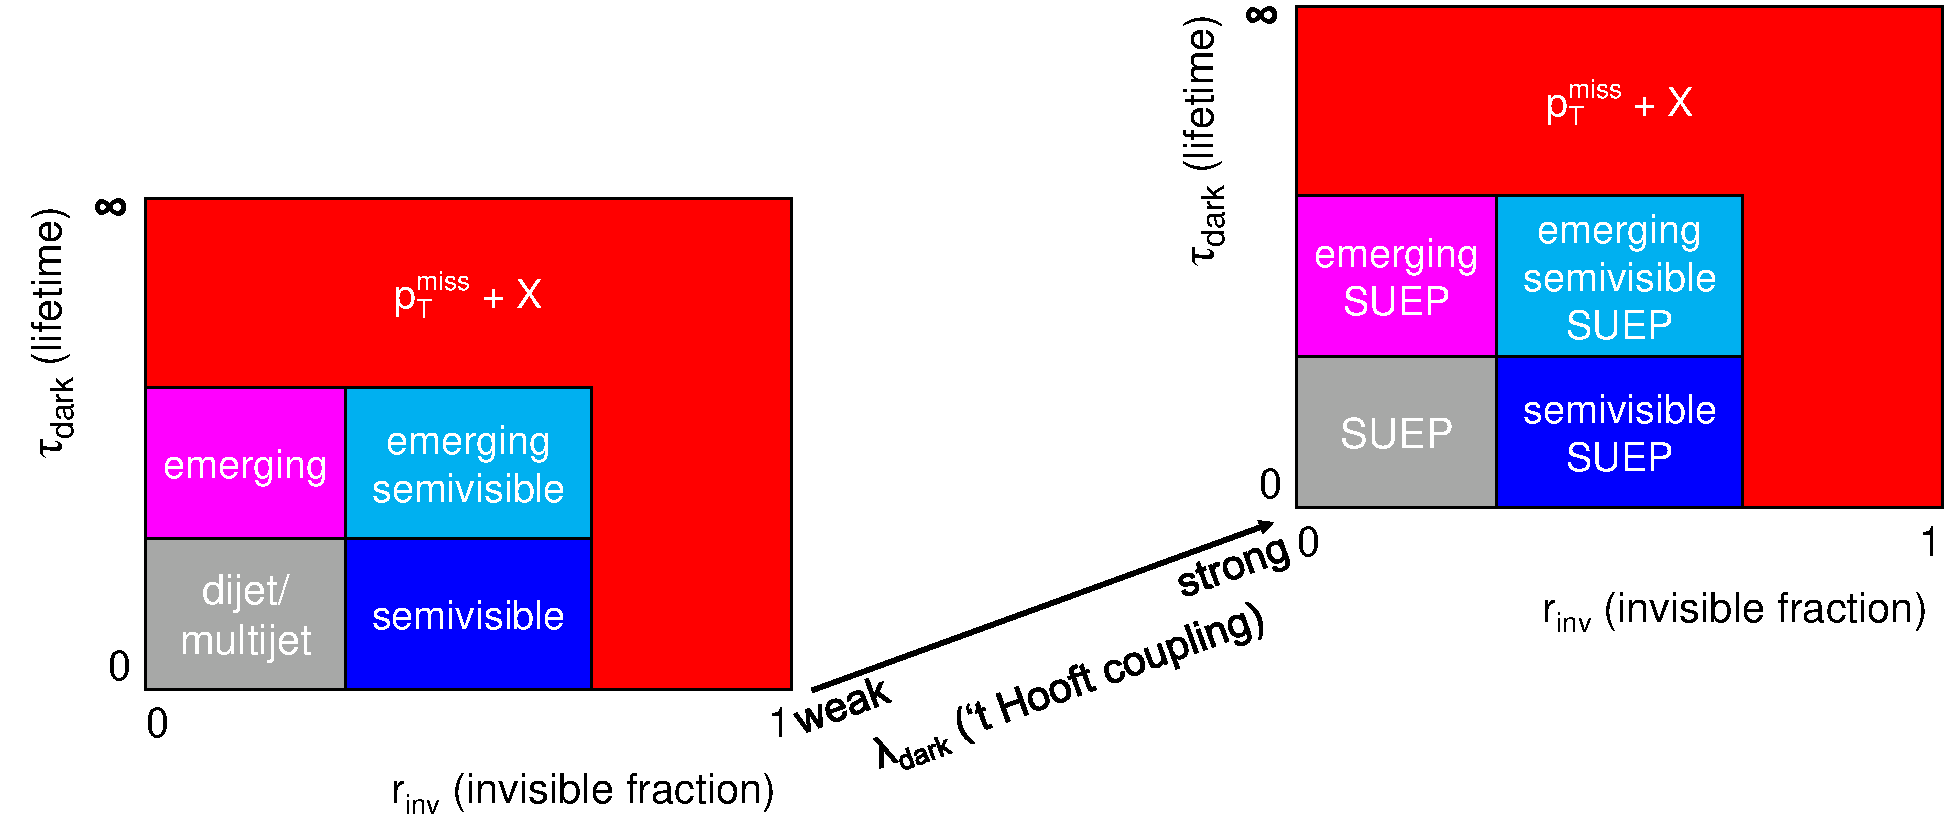
\includegraphics[width=0.95\myfigurewidth]{figures/svj_acceptance_diagram_v7.pdf}
\caption{A diagram illustrating the phenomenological signatures for different combinations of key dark QCD parameters.
For extreme values, the signatures resemble simpler models with multijets or \ptmiss; for intermediate values, the new phenomena become apparent.
}
\label{fig:svjacc}
\end{figure}

However, it is not required, or even necessarily likely, that each of these phenomena should appear in isolation.
\textbf{It is entirely possible that nature could produce semivisible emerging SUEPs or any other combination.}
Figure~\ref{fig:svjacc} illustrates the interplay between three characteristic parameters:
the dark meson lifetime $\taudark$, the invisible fraction $\rinv$, and the 't Hooft coupling \thooft.
For large values of \rinv and \taudark, the pre-existing searches for large \met would still be the most effective.
However, for intermediate values of those parameters, a dedicated strategy might outperform any of the individual searches noted above.
The best strategy for large values of \thooft in combination with the other parameters remains an open question,
while the generation of physically realistic events at intermediate \thooft has only recently become possible~\cite{Cesarotti:2020uod}.

All of these search strategies might need adjustments for other parameter variations,
such as the mediator masses and couplings and the various dark sector parameters discussed in Section~\ref{subsec:models}.
The most feasible way to explore this large parameter space is using a multidimensional scan,
similar to scans of the phenomenological minimal supersymmetric standard model (pMSSM)~\cite{Djouadi:1998di}
provided by CMS for earlier datasets~\cite{Khachatryan:2016nvf,SUS-16-033-supp} and currently in preparation for Run 2 by the PI and his colleagues.
Much like the pMSSM, this scan will include many random parameter combinations, with existing constraints included to eliminate models that are already ruled out.
We will reinterpret the latest dark QCD searches from LHC Runs 2 and 3 to understand which of these combined models are effectively excluded and which are not covered.
\textbf{Finding uncovered models will direct efforts to design new search strategies, including dedicated triggers, for the upcoming HL-LHC runs.}
The combined models will also help to further characterize any observed signal, which would likely have intermediate values of some parameters.

Obtaining the strongest results from the dark QCD scan relies on the success of the Run 3 SVJ search.
The proposed strategy includes several new elements, any of which may not converge on the necessary timescale.
However, each new element is independent from the others, and reasonable fallback options have been identified to mitigate these risks.
At minimum, the SVJ search will benefit from the use of the larger, higher energy Run 3 dataset.
Current searches do not exclude a \PZprime of mass 6\TeV, or alternatively \Pbifun with mass 3\TeV;
the discovery significance for these models will increase by a factor of 2.0--2.4.
This higher mass reach is driven primarily by the 80\% higher production cross section at $\sqrt{s}=13.6\TeV$ compared to 13\TeV.
Access to weaker processes with smaller coupling values, at all masses, will improve with the integrated luminosity of ${\sim}$190--260\fbinv compared to 138\fbinv.
\textbf{Given these risk mitigation strategies, we expect strong results from this search program.}
